

% ==========================================================================================
% 
%                                     LFC ERRORS
% 
% ==========================================================================================
% \section{LFC intensity errors}\label{appendix:LFC_errors} 

% \begin{SCfigure}[1][!ht]%
%     \begin{wide}  
%     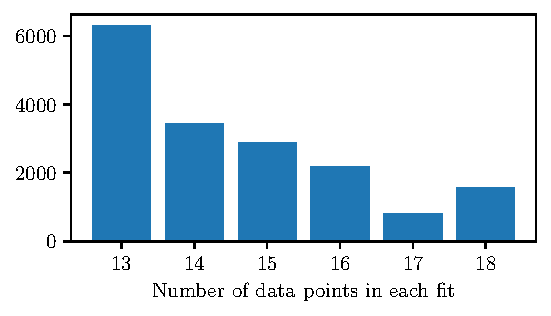
\includegraphics[scale=1]{figures/N_data_points.pdf}
%     \caption{Number of data points in each LFC peak fit, determined by the average distance between peaks in each order.}
%     \label{fig:N_data_points}
% \end{wide}
% \end{SCfigure}


% \begin{SCfigure}[1][!ht]%
%     \begin{wide}  
%     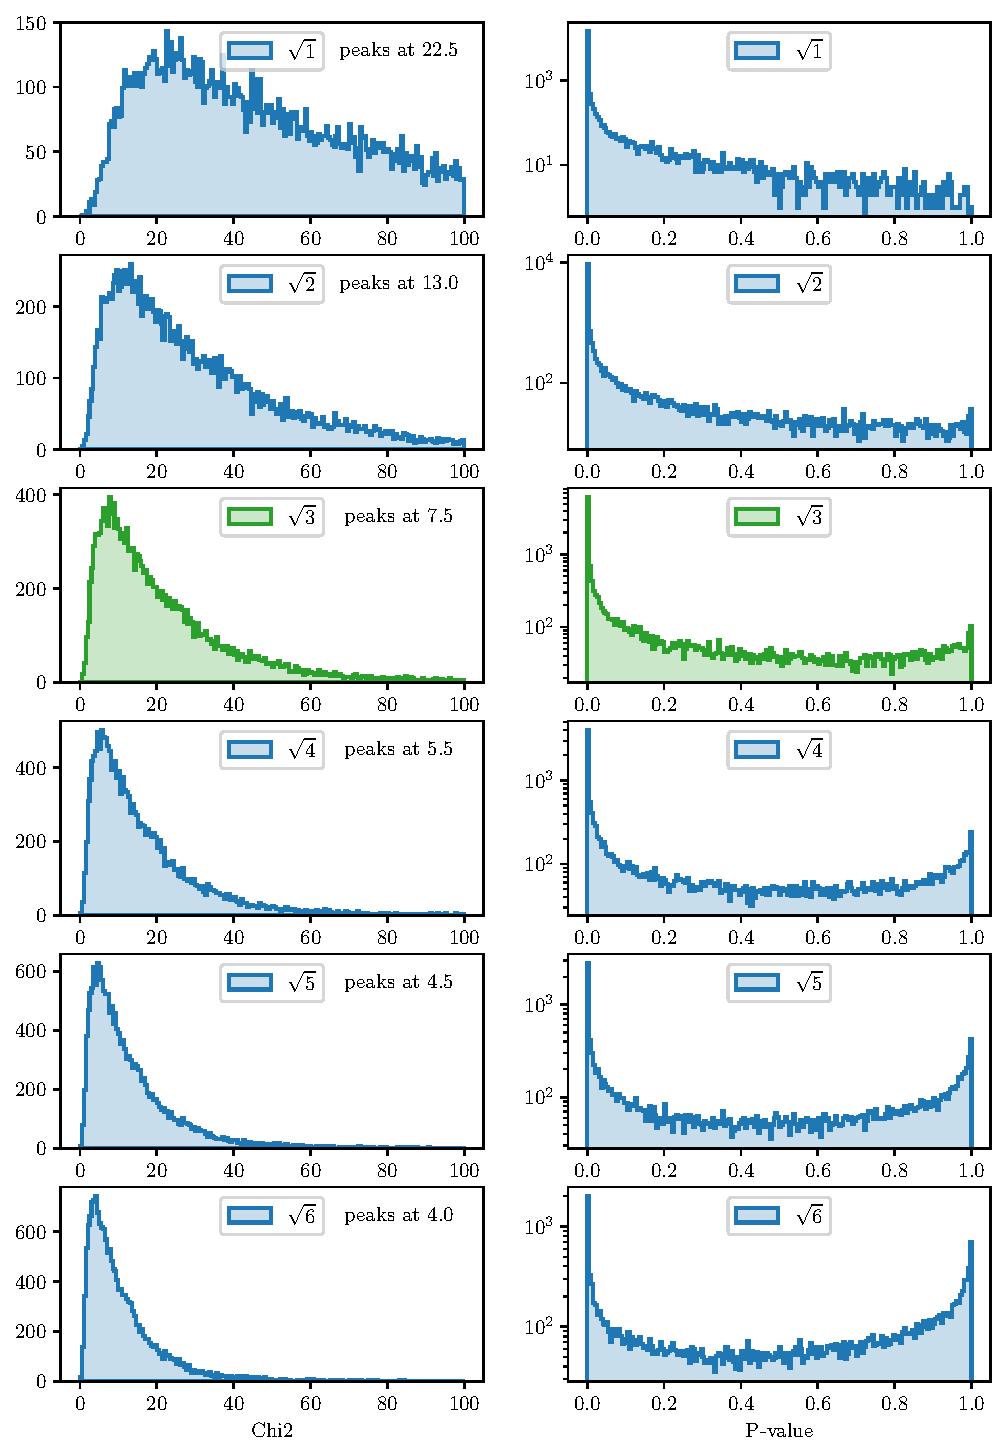
\includegraphics[scale=0.72]{figures/calib/calib_errors_extensive.pdf}
%     \caption{Chi2-values and P-values from individual LFC peak super-gauss fits with photon count (spectrum) errors multiplied by different scale-factors.}
%     \label{fig:calib_errors_extensive}
% \end{wide}
% \end{SCfigure}




% ==========================================================================================
% 
%                                     RV EXTRACTIONS
% 
% ==========================================================================================
\newpage
\section{RV extractions}\label{appendix:RV_extraction}

\begin{SCfigure}[1][!ht]%
    \begin{wide}  
    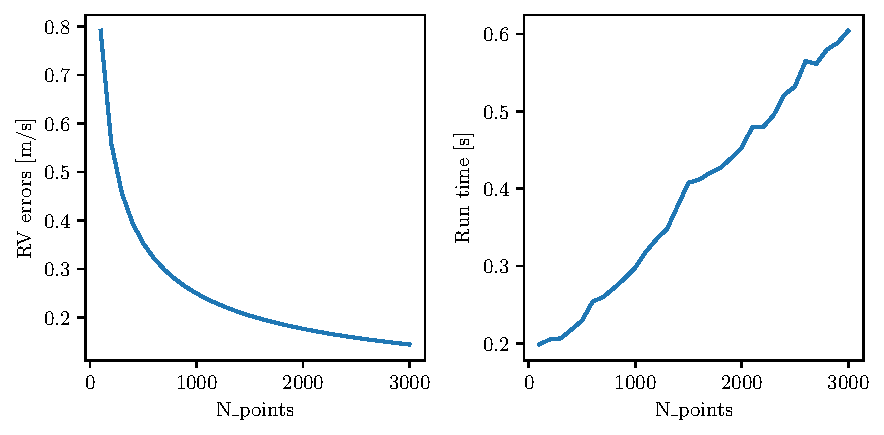
\includegraphics[scale=0.72]{figures/err_vs_run_time.pdf}
    \caption{Number of data points in each LFC peak fit, determined by the average distance between peaks in each order.}
    \label{fig:err_vs_run_time}
\end{wide}
\end{SCfigure}

% \begin{figure}[ht]
%     \centering
%     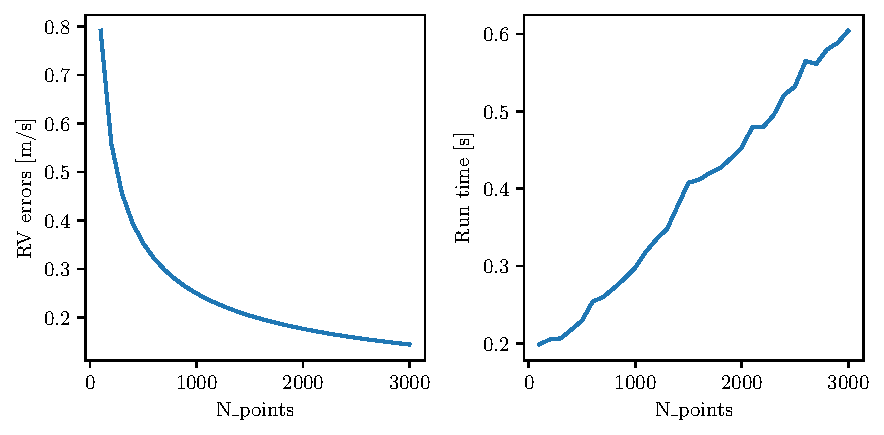
\includegraphics[scale=0.80]{figures/err_vs_run_time.pdf}
%     \caption{Number of data points in each LFC peak fit, determined by the average distance between peaks in each order.}
%     \label{fig:err_vs_run_time}
% \end{figure}


\begin{SCfigure}[1][!ht]%
    \begin{wide}  
    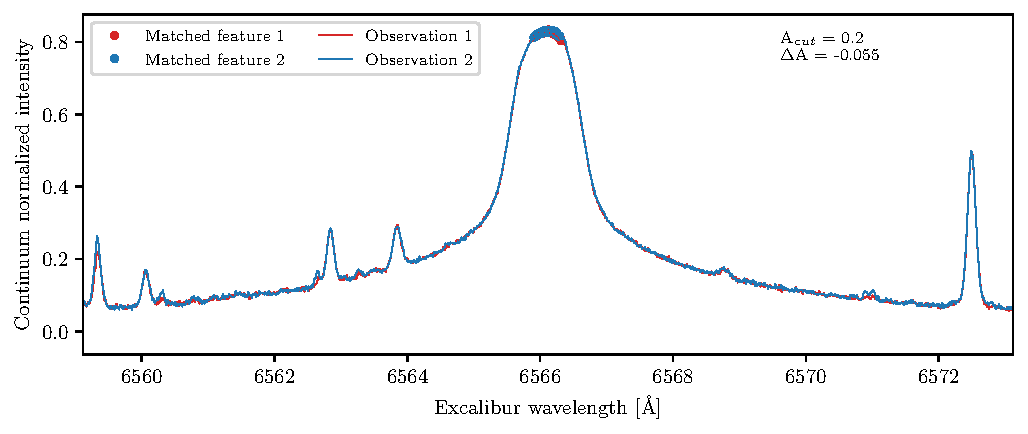
\includegraphics[scale=0.72]{figures/bad_match_example.pdf}
    \caption{Example of a bad match that made it through the filters. This match is actually correct, but yields a bad result because it is too broad for the standard data slice size.}
    \label{fig:bad_match_example}
\end{wide}
\end{SCfigure}

\subsection{Computational run times}\label{appendix:run_times} 
\todo{add number of function calls for the fitting}

\todo{add number of peak analyzed and so on}

\todo{add run times}

% ==========================================================================================
% 
%                                     RESULTS
% 
% ==========================================================================================
\newpage
\section{Results}\label{appendix:results}

\small{RV extracts from three more stars: HD 101501, HD 10700 and HD 26965. In each figure the top shows my final extracted RV shifts using excalibur calibrated, barycentric-corrected data (data column \texttt{bary\char`_excalibur}), the center shows Lily Zhao et al's results using a chunk-by-chunk (CBC) analysis technique \cite{yale_data}, and the bottom shows residuals from subtracting Lily's results from mine. }

\begin{SCfigure}[1][!ht]%
    \begin{wide}  
    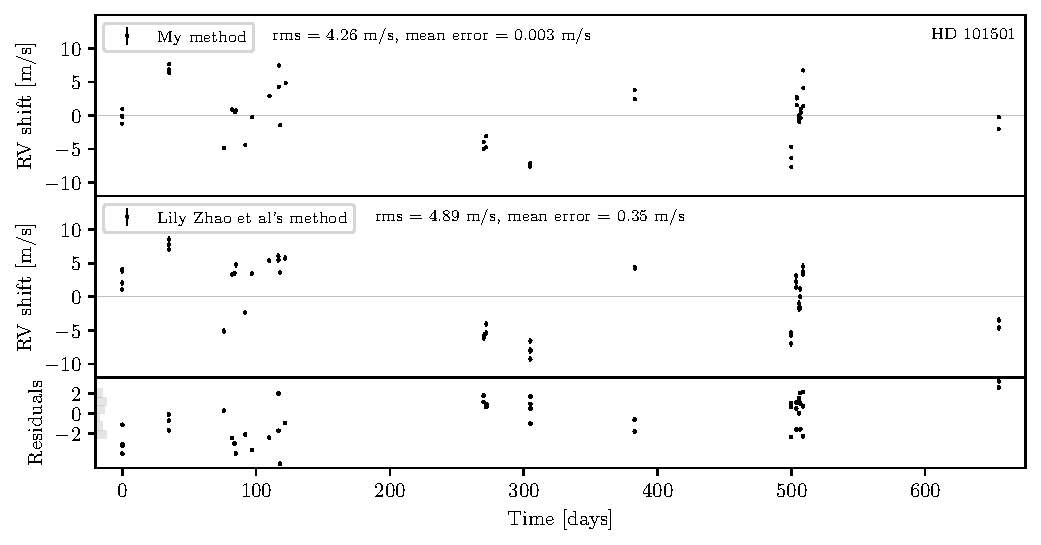
\includegraphics[width=\textwidth]{figures/HD101501_barycentric_rv_vs_lily.pdf}
    \caption{HD 101501\newline 45 observations made between 2019-2-10 and 2020-11-26.}
    \label{fig:HD101501_rvs}
\end{wide}
\end{SCfigure}

\vspace{-0.75cm}

\begin{SCfigure}[1][!ht]%
    \begin{wide}  
    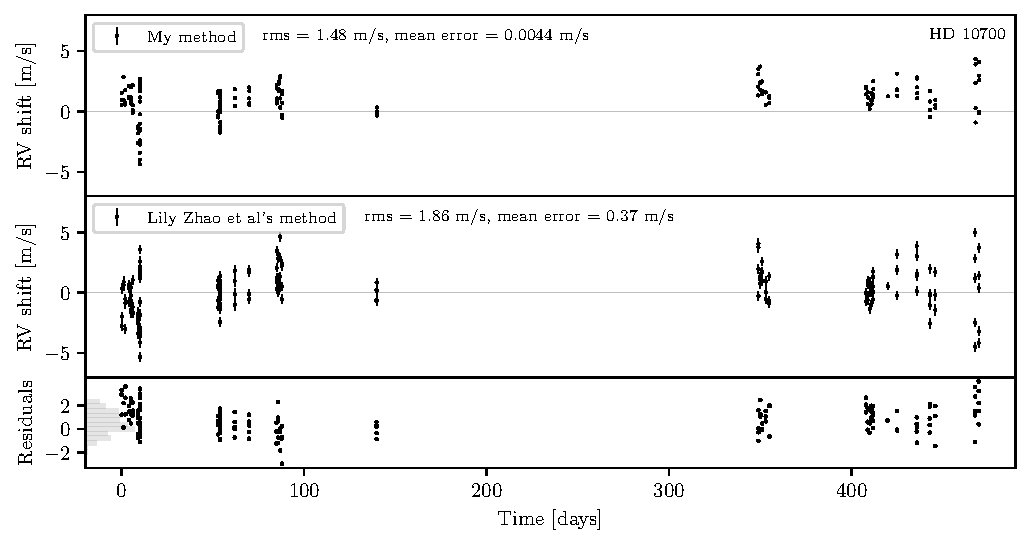
\includegraphics[width=\textwidth]{figures/HD10700_barycentric_rv_vs_lily.pdf}
    \caption{HD 10700\newline 174 observations made between 2019-8-15 and 2020-11-27.}
    \label{fig:HD10700_rvs}
\end{wide}
\end{SCfigure}

\vspace{-0.75cm}

\begin{SCfigure}[1][!ht]%
    \begin{wide}  
    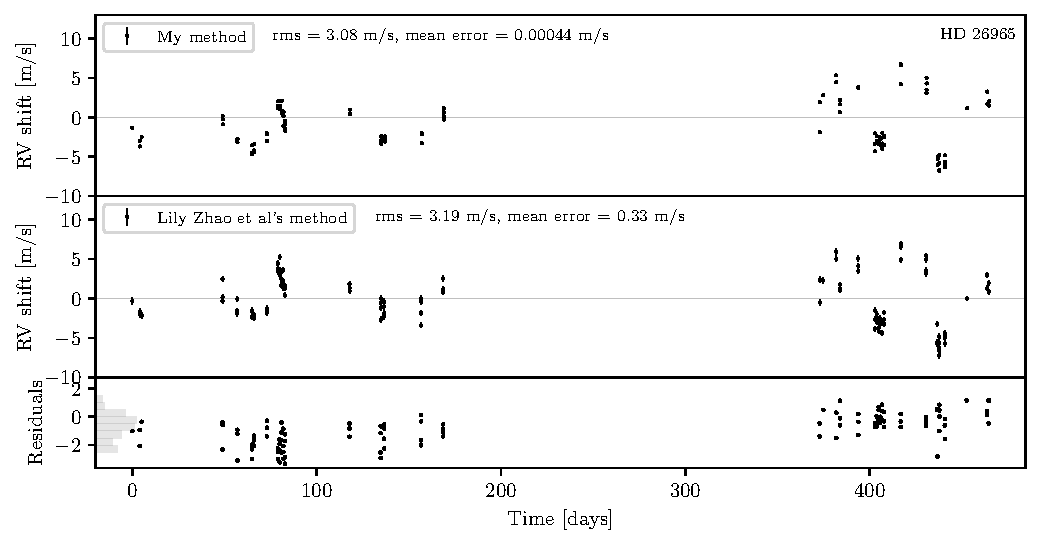
\includegraphics[width=\textwidth]{figures/HD26965_barycentric_rv_vs_lily.pdf}
    \caption{HD 26965\newline 114 observations made between 2019-8-20 and 2020-11-27.}
    \label{fig:HD26965_rvs}
\end{wide}
\end{SCfigure}
